%%%%%%%%%%%%%%%%%%%%%%%%%%%%%%%%%%%%%%%%%%%%%%%%%%%%%%
% PREAMBLE
%%%%%%%%%%%%%%%%%%%%%%%%%%%%%%%%%%%%%%%%%%%%%%%%%%%%%%
\documentclass[xcolor=x11names, compress]{beamer}

%% General document %%%%%%%%%%%%%%%%%%%%%%%%%%%%%%%%%%
\usepackage{graphicx}
\usepackage{booktabs}
\usepackage{caption}

%% Beamer Layout %%%%%%%%%%%%%%%%%%%%%%%%%%%%%%%%%%%%%
\useoutertheme[subsection=false,shadow]{miniframes}
\useinnertheme{default}
\usefonttheme{serif}
\usepackage{palatino}
\usepackage{hyperref}
%\usepackage{mwe}

\setbeamerfont{title like}{shape=\scshape}
\setbeamerfont{frametitle}{shape=\scshape}

\setbeamercolor*{lower separation line head}{bg=DeepSkyBlue4} 
\setbeamercolor*{normal text}{fg=black,bg=white} 
\setbeamercolor*{alerted text}{fg=red} 
\setbeamercolor*{example text}{fg=black} 
\setbeamercolor*{structure}{fg=black} 
\setbeamertemplate{blocks}[rounded][shadow=true]
\setbeamercolor*{block title}{fg= white,bg= gray}
\setbeamercolor*{block body}{fg= black,bg= gray!20}
 
\setbeamercolor*{palette tertiary}{fg=black,bg=black!10} 
\setbeamercolor*{palette quaternary}{fg=black,bg=black!10} 

\renewcommand{\(}{\begin{columns}}
\renewcommand{\)}{\end{columns}}
\newcommand{\<}[1]{\begin{column}{#1}}
\renewcommand{\>}{\end{column}}

\begin{document}

%%%%%%%%%%%%%%%%%%%%%%%%%%%%%%%%%%%%%%%%%%%%%%%%%%%%%%
% TITLE PAGE

\title[]{\LARGE{Multi-scale models for biogeography}} 
\author{\normalsize{Petr Keil}} % Your name
	\date{}
\institute
{
	\normalsize{Center for Theoretical Study, Charles University in Prague, 
	Czech Republic}
}
\begin{frame}
    \begin{figure}
       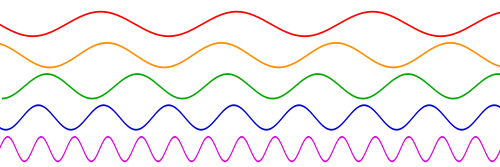
\includegraphics[height=0.15\linewidth]{fig/freq.png}
    \end{figure} 
	\titlepage % Print the title page as the first slide
    %\centerline{\textit{pkeil@seznam.cz}}
\end{frame}

% -----------------------------------------------------------------------------

\begin{frame}

\begin{figure}
	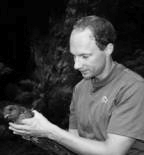
\includegraphics[height=0.2\linewidth]{fig/walter.png}
	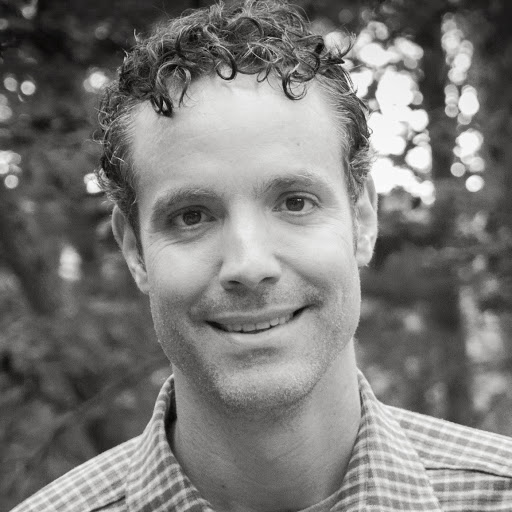
\includegraphics[height=0.2\linewidth]{fig/adam.png}
	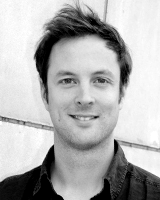
\includegraphics[height=0.2\linewidth]{fig/hugh.png}
	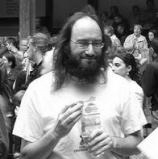
\includegraphics[height=0.2\linewidth]{fig/bob.png}
	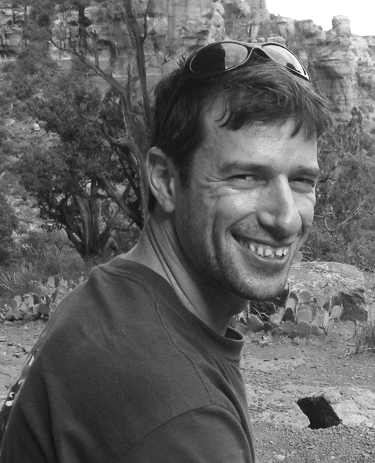
\includegraphics[height=0.2\linewidth]{fig/jonathan.png}
\end{figure}

\textbf{Walter Jetz}, Yale University 

\textbf{Adam M. Wilson}, Yale University 

\textbf{Hugh Sturrock}, UC San Francisco 

\textbf{Bob O'Hara}, Bik-F Frankfurt 

\textbf{Jonathan Belmaker}, Tel Aviv University


\end{frame}

%%%%%%%%%%%%%%%%%%%%%%%%%%%%%%%%%%%%%%%%%%%%%%%%%%%%%%%%%%%%%%%%%%%%%%%%%%%%%%
\section{What is a multi-scale model?}
\subsection{}
\begin{frame}
	\Large{Part 1: \insertsection}
\end{frame}
%%%%%%%%%%%%%%%%%%%%%%%%%%%%%%%%%%%%%%%%%%%%%%%%%%%%%%%%%%%%%%%%%%%%%%%%%%%%%%

\begin{frame}
\frametitle{Single-scale statistical model}
\begin{figure}
	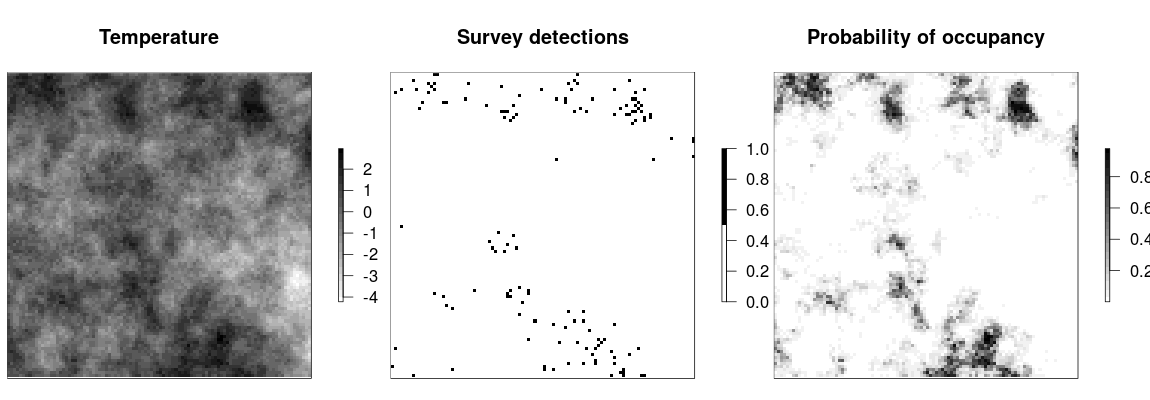
\includegraphics[width=1\linewidth]{fig/maps_single.png}
\end{figure}

\end{frame}

% -----------------------------------------------------------------------------

\begin{frame}
\frametitle{Single-scale statistical model}
\begin{figure}
	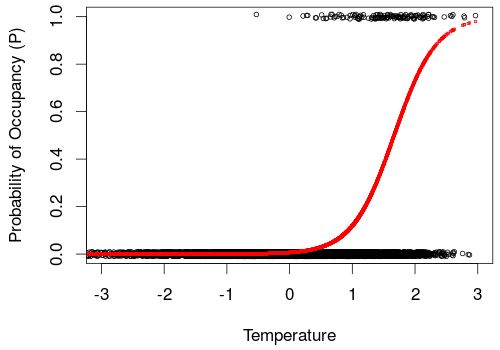
\includegraphics[width=0.7\linewidth]{fig/logistic.png}
\end{figure}
\begin{equation}
	logit (P_{i}) = \beta_0 + \beta_1 Temperature_{i}
\end{equation}
\begin{equation}
	O_i \sim Bernoulli(P_i)
\end{equation}

\end{frame}

% -----------------------------------------------------------------------------

\begin{frame}
\frametitle{Response finer than predictors}
\begin{figure}
	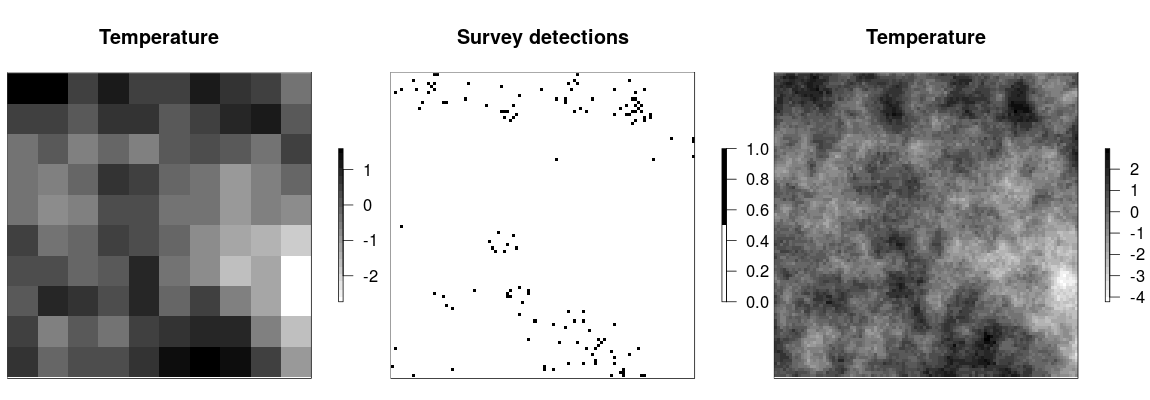
\includegraphics[width=1\linewidth]{fig/maps_multiII.png}
\end{figure}

\footnotesize{McInerny \& Purves (2011) \textit{Methods in Ecology and Evolution}}
\end{frame}

% -----------------------------------------------------------------------------

\begin{frame}
\frametitle{Predictor finer than response}
\begin{figure}
	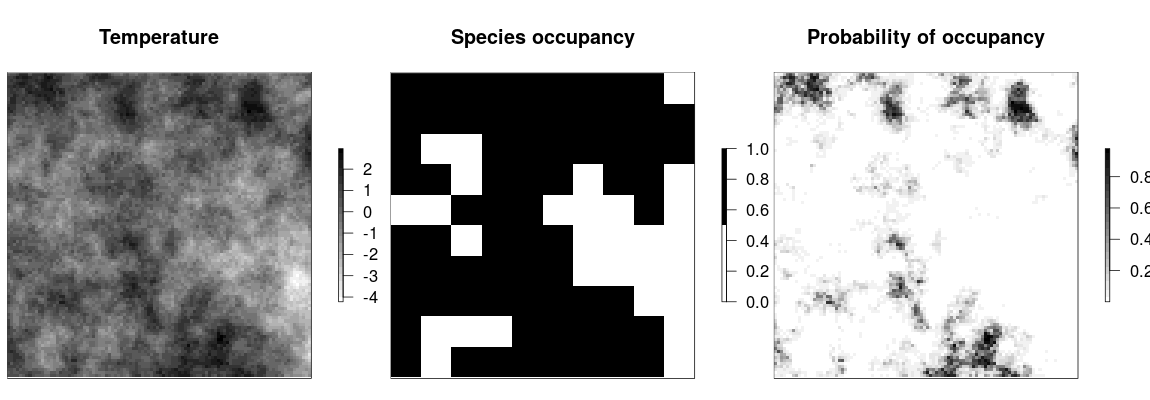
\includegraphics[width=1\linewidth]{fig/maps_multiI.png}
\end{figure}

\footnotesize{Keil \textit{et al.} (2013) \textit{Methods in Ecology and Evolution} }

\footnotesize{Keil \textit{et al.} (2014) \textit{Diversity \& Distributions} }

\footnotesize{Keil \& Jetz (2014) \textit{Ecological Applications} }

\footnotesize{Sturrock \textit{et al.} (2015) \textit{Malaria Journal}}

\end{frame}


% -----------------------------------------------------------------------------

\section{How does it work?}
\subsection{}
\begin{frame}
	\Large{Part 2: \insertsection}
\end{frame}

% ----------------------------------------------------------------------------
\begin{frame}
\frametitle{2-scale logistic model for one species}
\begin{figure}
	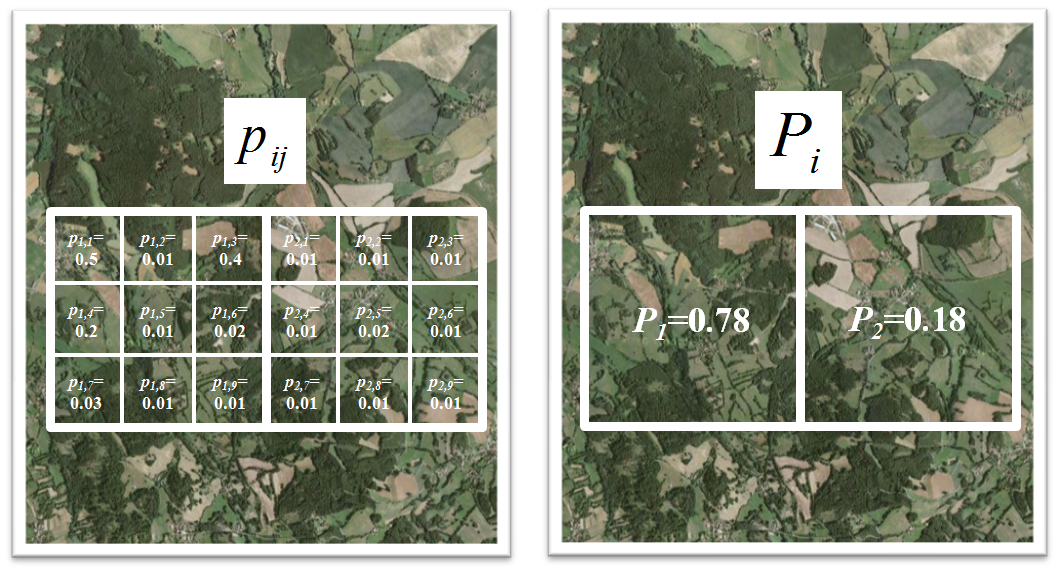
\includegraphics[width=0.7\linewidth]{fig/scalingp2.png}
\end{figure}
\footnotesize{
\uncover<1->
{
\begin{equation}
logit (p_{ij}) = \beta_0 + \beta_1 Temperature_{ij}
\end{equation}
}
\uncover<2->
{
\begin{equation}
P_i=1- \prod_{j=1}^n{(1-p_{ij})} 
\end{equation}
}
\uncover<3->
{
\begin{equation}
O_{i} \sim Bernoulli(P_i) 
\end{equation}
}
}
\let\thefootnote\relax\footnote{Keil \textit{et al.} 2013 \textit{Methods in Ecology and Evolution}}

\end{frame}

% -----------------------------------------------------------------------------
\begin{frame}
\frametitle{2-scale Poisson model of species richness}


\begin{figure}
	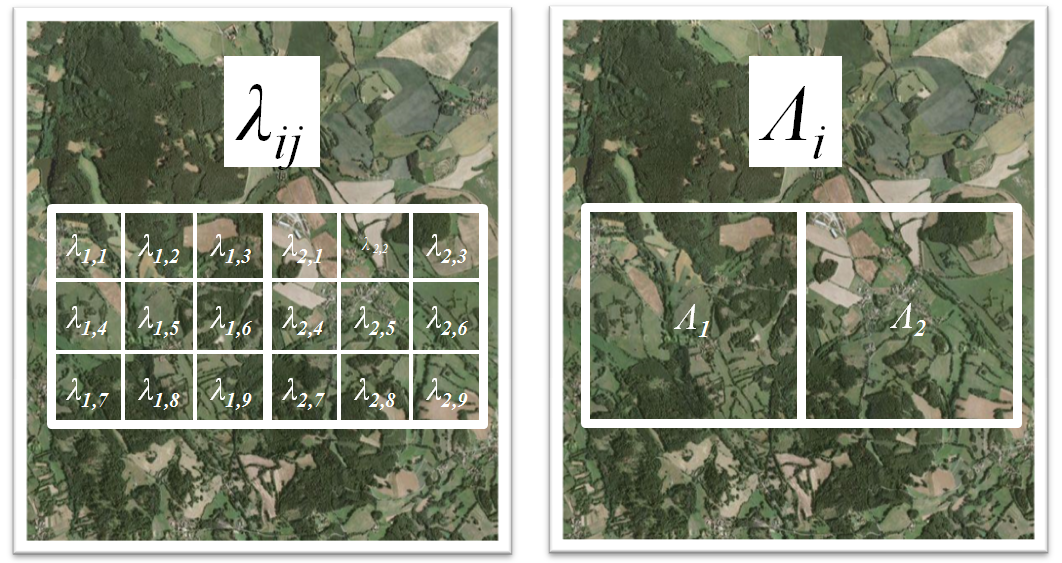
\includegraphics[width=0.65\linewidth]{fig/scalings1.png}
\end{figure}

\uncover<1->{
\footnotesize{
\begin{equation}
\lambda_{ij} = f(environment_{ij})
\end{equation}

\begin{equation}
\Lambda_i = \beta_w \times \hat{\lambda_i}
\end{equation}

\begin{equation}
S_{i} \sim Poisson(\Lambda_i)
\end{equation}

}}

\let\thefootnote\relax\footnote{Keil \& Jetz 2014 \textit{Ecological Applications}}
\end{frame}

% ----------------------------------------------------------------------------
\begin{frame}
\frametitle{How do we fit these models?}

\begin{itemize}[<+(1)->]
	\item Likelihood maximization
	\item MCMC (Markov Chain Monte Carlo)
	\item INLA (Integrated Nested Laplace Approximation)
	\item \textbf{Steep learning curve}
\end{itemize}

\end{frame}

%%%%%%%%%%%%%%%%%%%%%%%%%%%%%%%%%%%%%%%%%%%%%%%%%%%%%%%%%%%%%%%%%%%%%%%%%%%%%%
\section{Case studies}
\subsection{}
\begin{frame}
	\Large{Part 3: \insertsection}
\end{frame}
%%%%%%%%%%%%%%%%%%%%%%%%%%%%%%%%%%%%%%%%%%%%%%%%%%%%%%%%%%%%%%%%%%%%%%%%%%%%%%
% ----------------------------------------------------------------------------
\begin{frame}
\frametitle{Case study 1 -- Single-species}
\begin{figure}
	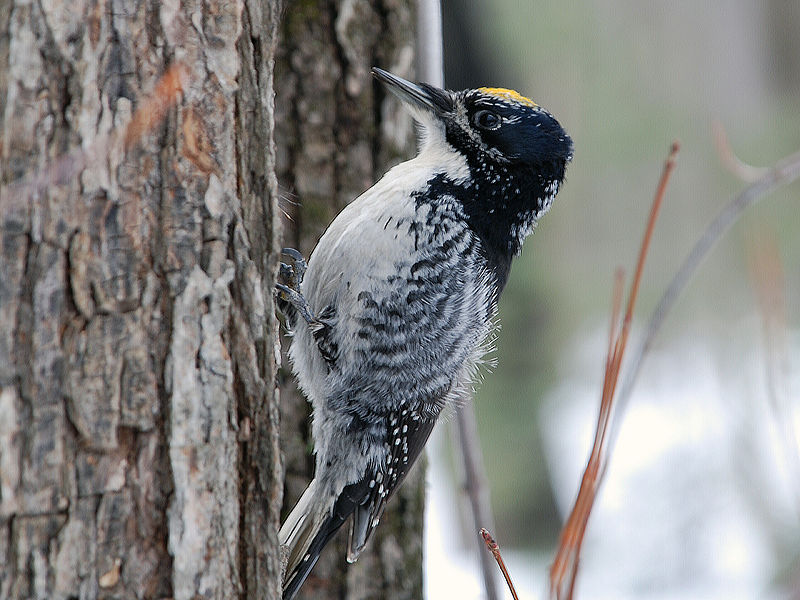
\includegraphics[width=0.25\linewidth]{fig/woodpecker.png}
\end{figure}
\centerline{American three-toed woodpecker (\textit{Picoides dorsalis}, Baird 1858)}

\begin{figure}
	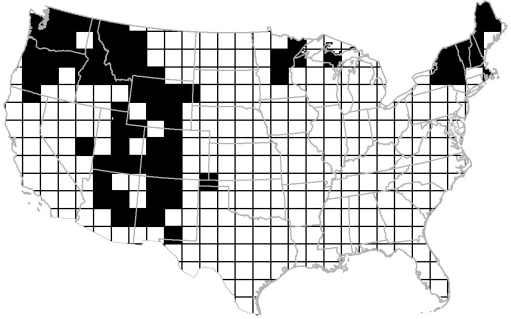
\includegraphics[width=0.35\linewidth]{fig/presabs.png}
	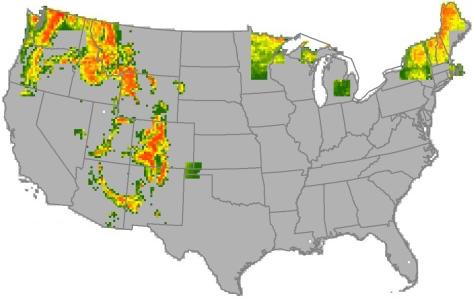
\includegraphics[width=0.35\linewidth]{fig/model1.png}
	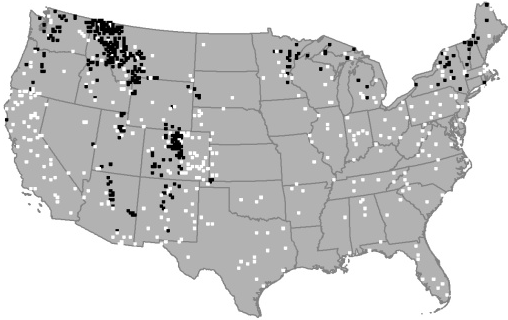
\includegraphics[width=0.35\linewidth]{fig/validation.png}
\end{figure}
\centerline{$AUC$=0.93; Nagelkerke's $R^2$ = 0.69}

\let\thefootnote\relax\footnote{Keil \textit{et al.} 2014 \textit{Diversity \& Distributions}}
\end{frame}

% ----------------------------------------------------------------------------

\begin{frame}
\frametitle{Case study 2 -- Species richness of birds}
\begin{figure}
	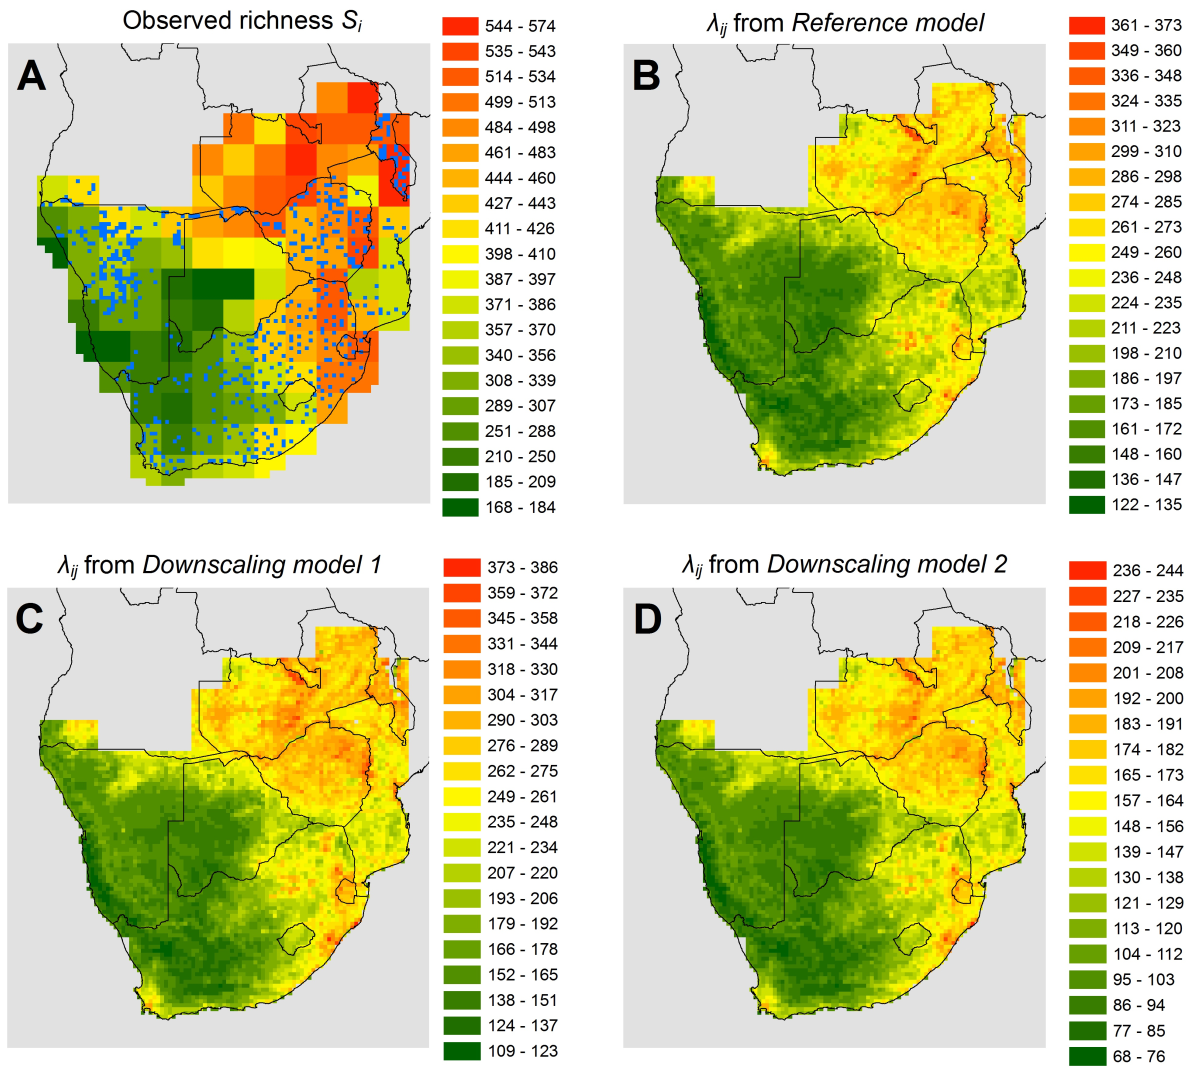
\includegraphics[width=0.7\linewidth]{fig/afr_coarse.png}
\end{figure}
\let\thefootnote\relax\footnote{Keil \textit{et al.} 2014 \textit{Ecological Applications}}
\end{frame}

% -----------------------------------------------------------------------------
\begin{frame}
\frametitle{Case study 3 - Species richness of butterflies}
\begin{figure}
	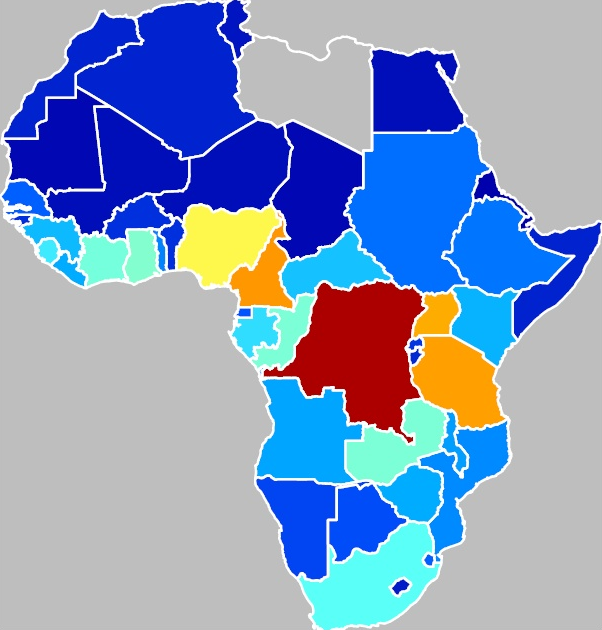
\includegraphics[height=0.4\linewidth]{fig/afr_checklists.png}
	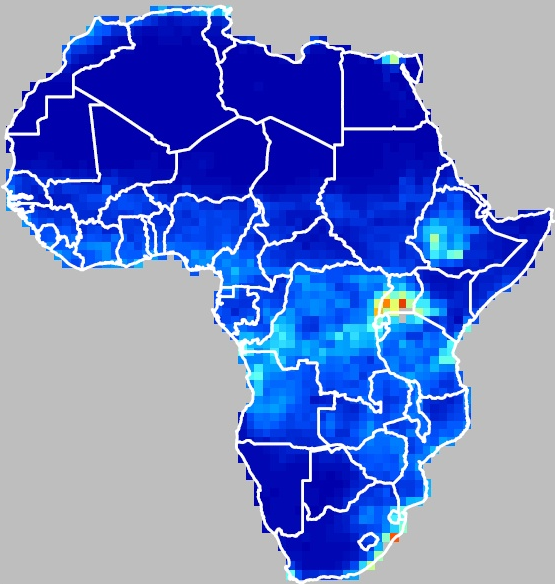
\includegraphics[height=0.4\linewidth]{fig/afr_results.png}
	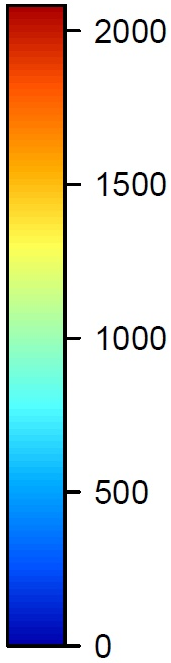
\includegraphics[height=0.4\linewidth]{fig/scale.png}
\end{figure}

\let\thefootnote\relax\footnote{\textit{Unpublished}}

% -----------------------------------------------------------------------------
\end{frame}
\begin{frame}{Case study 4 -- Malaria in Swaziland}
	\begin{figure}
		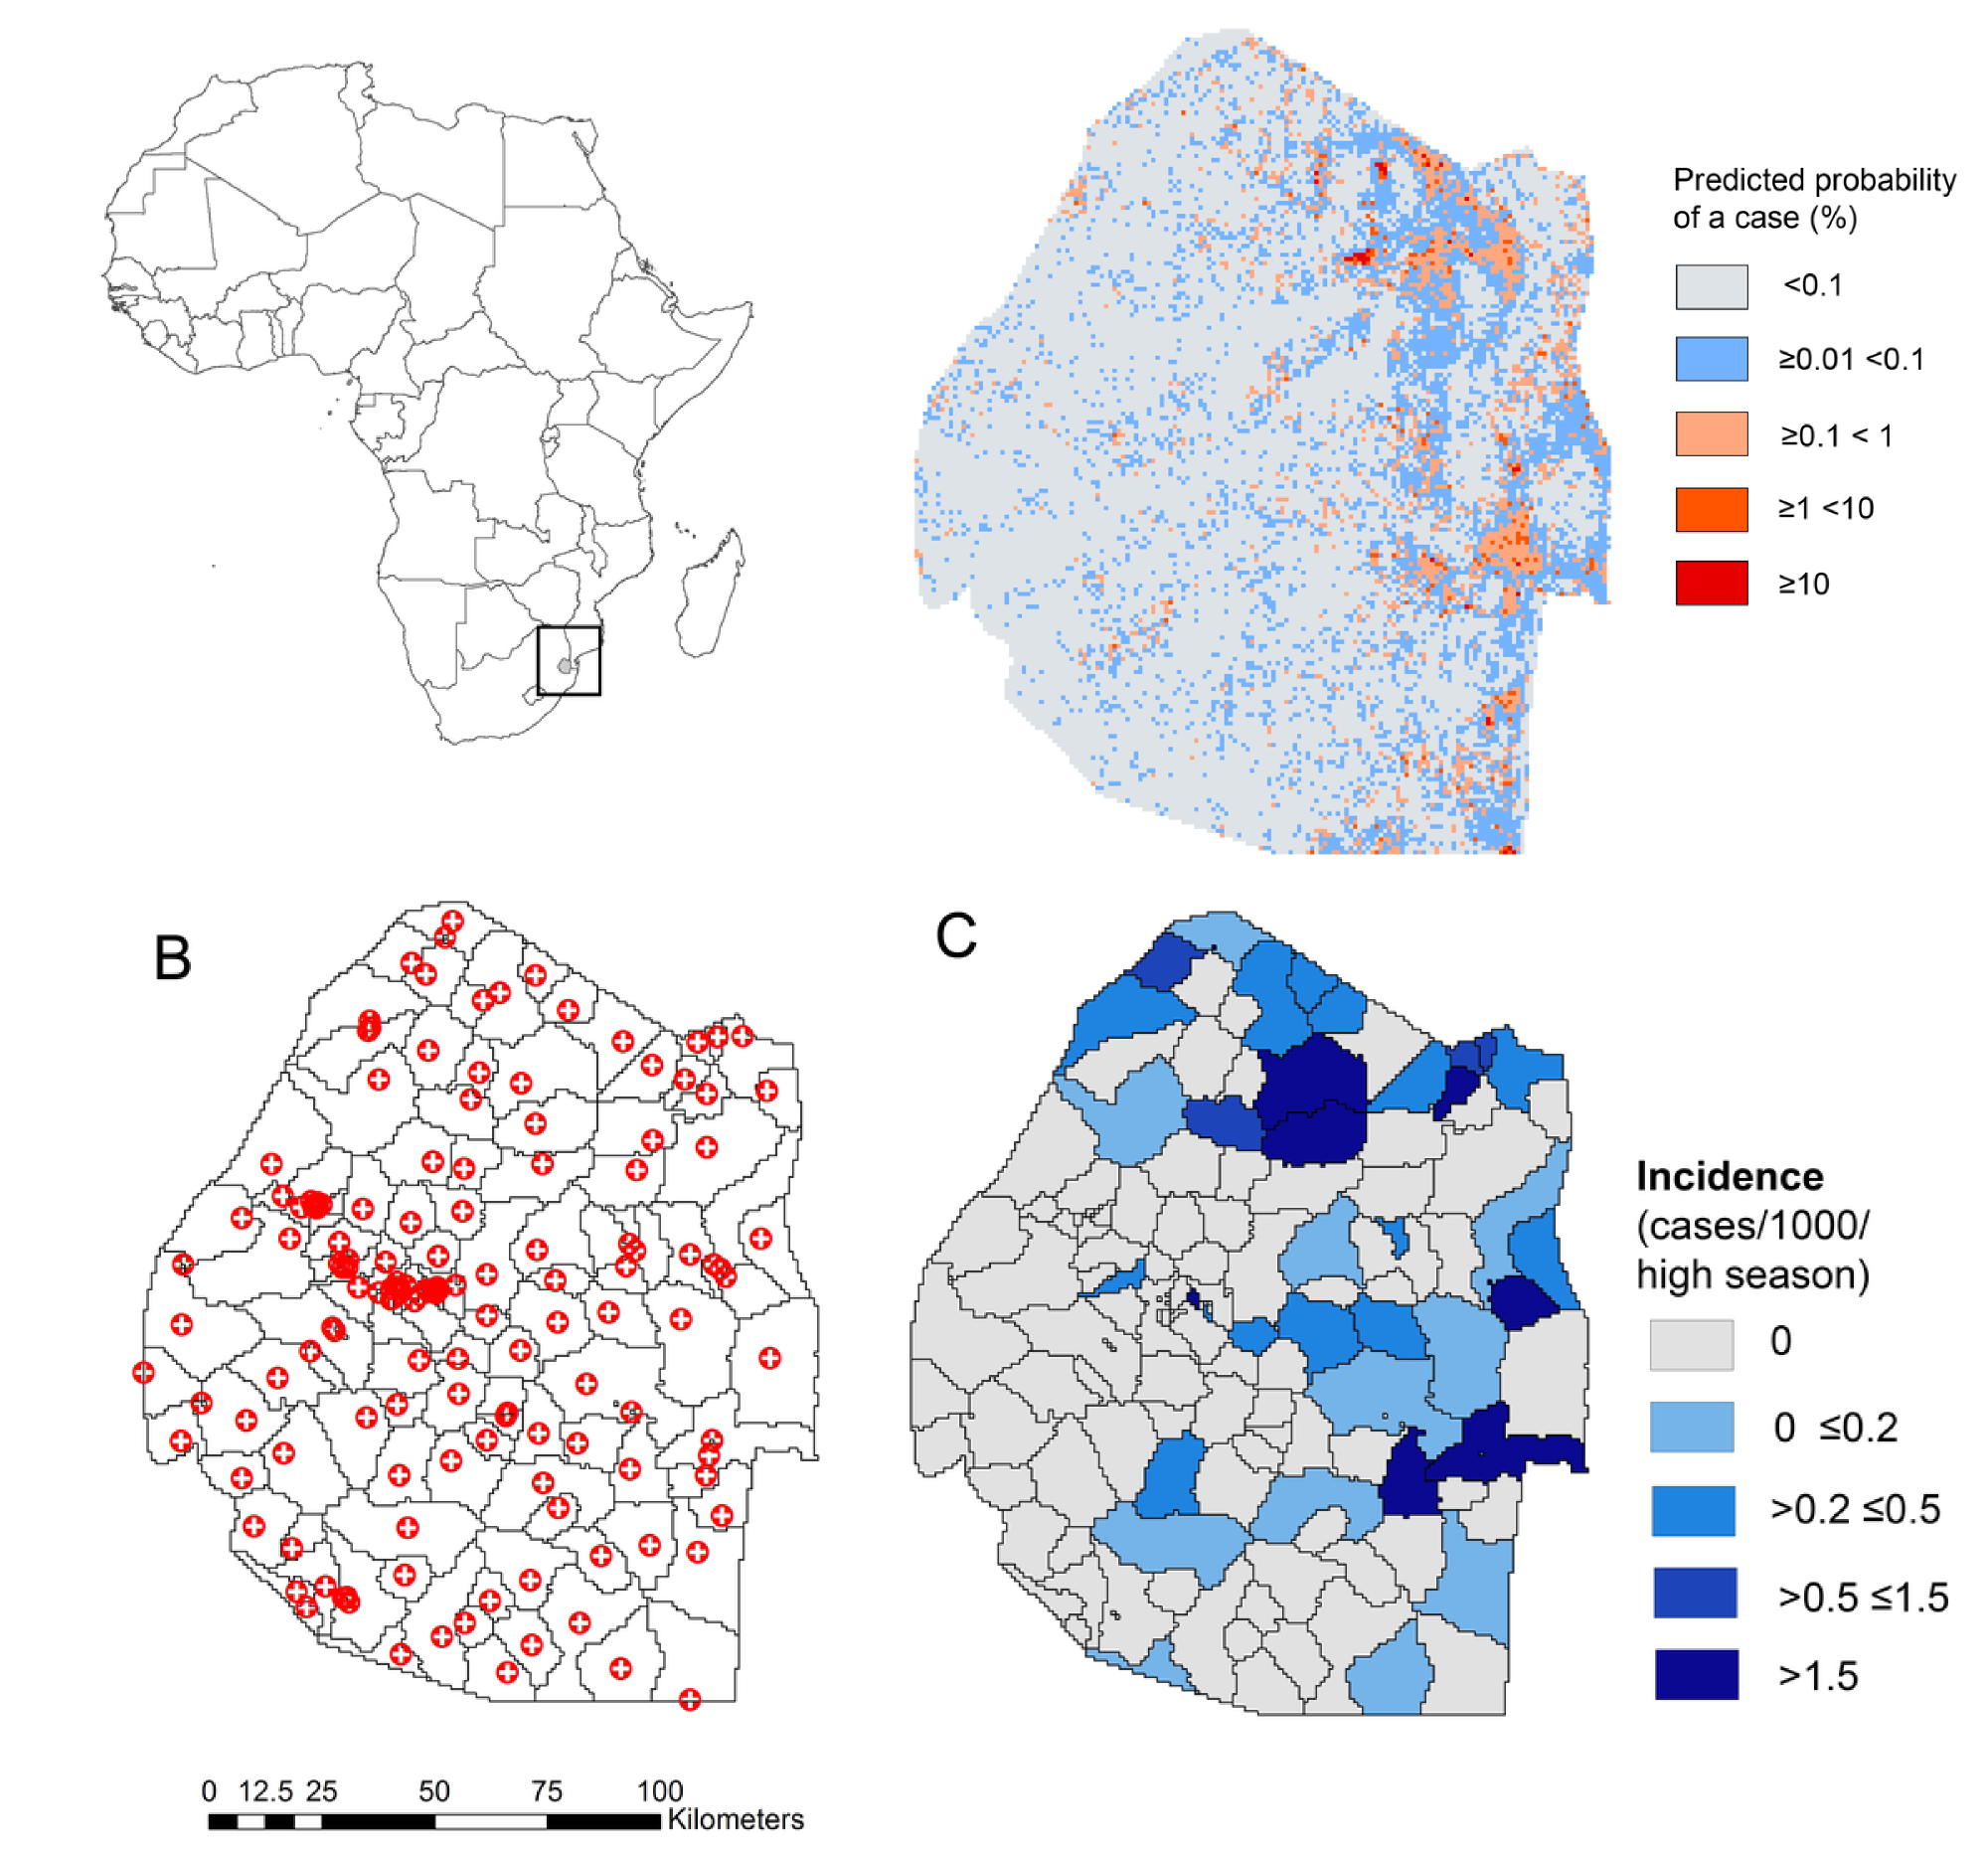
\includegraphics[height=2.5in]{fig/swazi_results.png}  
	\end{figure}
	\let\thefootnote\relax\footnote{Sturrock \textit{et al.} (2015) \textit{Malaria Journal}}
\end{frame}

%%%%%%%%%%%%%%%%%%%%%%%%%%%%%%%%%%%%%%%%%%%%%%%%%%%%%%%%%%%%%%%%%%%%%%%%%%%%%%
\section{Future prospects}
\subsection{}
\begin{frame}
	\Large{Part 4: \insertsection}
\end{frame}
%%%%%%%%%%%%%%%%%%%%%%%%%%%%%%%%%%%%%%%%%%%%%%%%%%%%%%%%%%%%%%%%%%%%%%%%%%%%%%

\begin{frame}
\frametitle{Linking GLM, point processes and MaxEnt}
\begin{figure}
   \raisebox{.5\height}{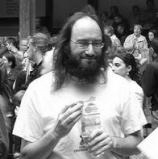
\includegraphics[height=0.2\linewidth]{fig/bob.png}}
	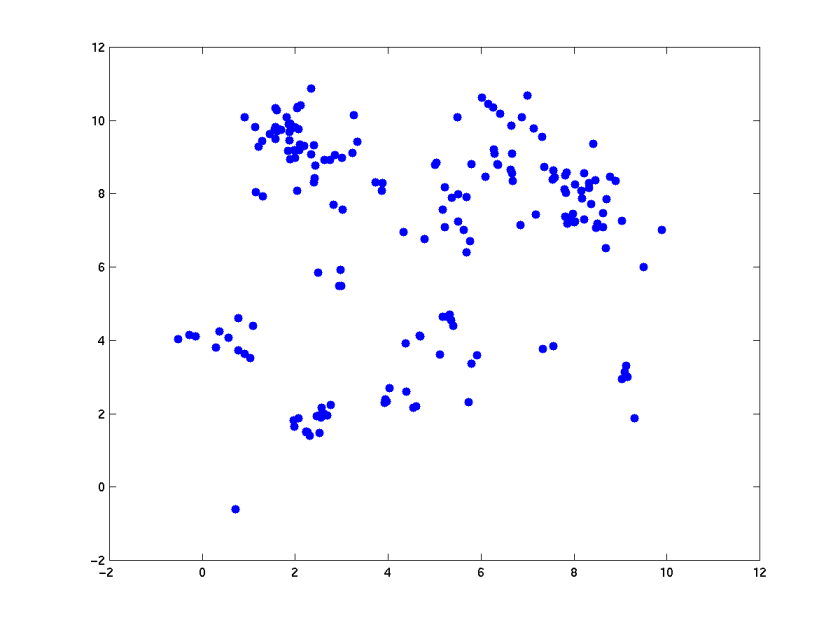
\includegraphics[height=0.4\linewidth]{fig/point_process.png}
\end{figure}
\centerline{Bob O'Hara}
\let\thefootnote\relax\footnote{Renner \& Warton (2013) \textit{Biometrics}}
\end{frame}


% ----------------------------------------------------------------------------
\begin{frame}
\frametitle{From grids to \textbf{continuous scale}}
\begin{figure}
	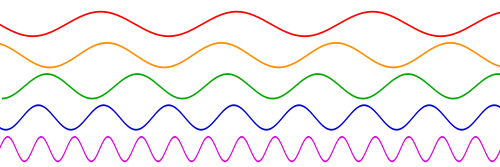
\includegraphics[height=0.3\linewidth]{fig/freq.png}
\end{figure}
Keywords: Fourirer transform, Wavelets, eigenvector maps, ...
\let\thefootnote\relax\footnote{Sandel (2015) \textit{Ecography}}
\end{frame}


% ----------------------------------------------------------------------------

\begin{frame}
\frametitle{The idea of \textbf{fundamental scale}}

\begin{figure}
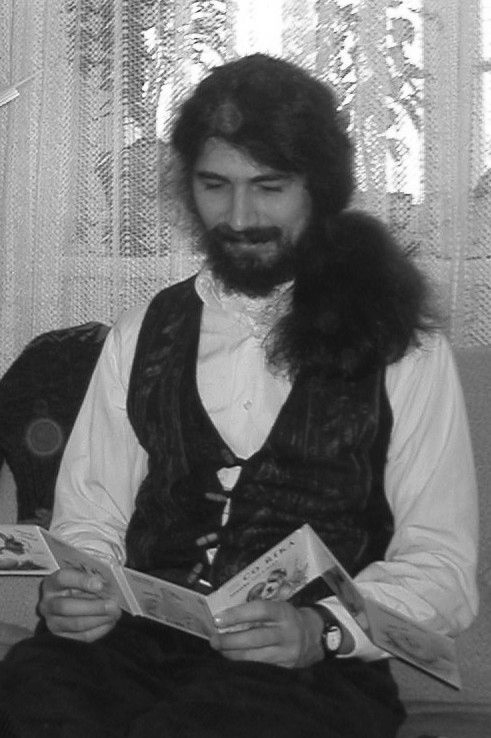
\includegraphics[height=0.3\linewidth]{fig/arnost.png}
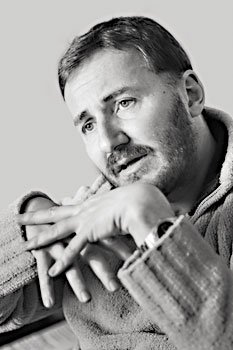
\includegraphics[height=0.3\linewidth]{fig/david.png}
\end{figure}
\centerline{Arnost L. Sizling, David Storch}

\let\thefootnote\relax\footnote{Sizling \textit{et al.} (2009) \textit{PNAS}; Storch \& Sizling (2008) \textit{Folia Geobotanica}}

\end{frame}


%%%%%%%%%%%%%%%%%%%%%%%%%%%%%%%%%%%%%%%%%%%%%%%%%%%%%%%%%%%%%%%%%%%%%%%%%%%%%%
\section{Summary}
\subsection{}
%%%%%%%%%%%%%%%%%%%%%%%%%%%%%%%%%%%%%%%%%%%%%%%%%%%%%%%%%%%%%%%%%%%%%%%%%%%%%%

\begin{frame}
\frametitle{Summary}
\begin{itemize}[<+(1)->]
\item We can fit models using data from disparate grains without having to loose data.
\item We can downscale maps.
\item We can derive fine-scale niche using coarse-scale environmental data.
\item There are exciting opportunities for research projects.
\item The tools need to be made more accessible.
\end{itemize}
\end{frame}

% ----------------------------------------------------------------------------

\begin{frame}
\frametitle{Acknowledgements}
\begin{figure}
	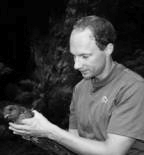
\includegraphics[height=0.2\linewidth]{fig/walter.png}
	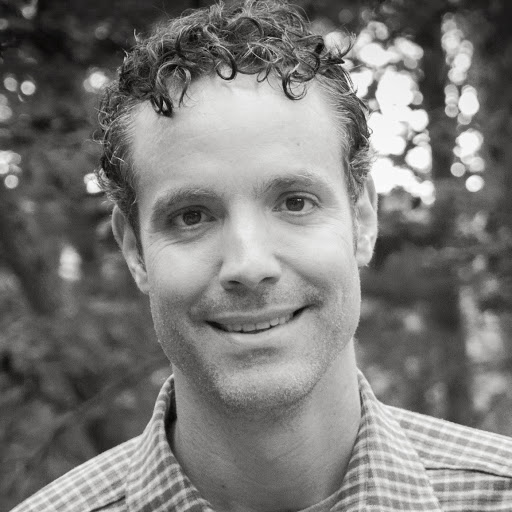
\includegraphics[height=0.2\linewidth]{fig/adam.png}
	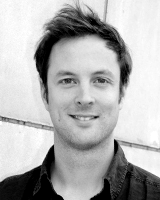
\includegraphics[height=0.2\linewidth]{fig/hugh.png}
	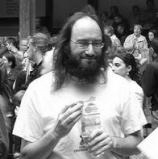
\includegraphics[height=0.2\linewidth]{fig/bob.png}
	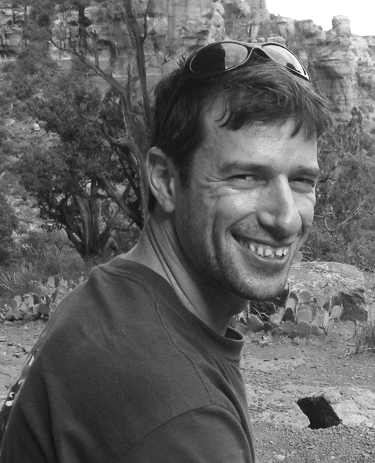
\includegraphics[height=0.2\linewidth]{fig/jonathan.png}
\end{figure}
\footnotesize{
\centerline{Walter Jetz, Adam M. Wilson, Hugh Sturrock, Bob O'Hara, Jonathan Belmaker}}

\begin{figure}
	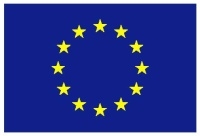
\includegraphics[height=0.15\linewidth]{fig/eu.jpg}
	
\includegraphics[height=0.15\linewidth]{fig/fp7.jpg}
\end{figure}
\footnotesize{
I received funding from People Programme (\textbf{Marie Curie Actions}) of the European Union’s Seventh Framework Programme (FP7/2007-2013) under REA grant agreement no 302868.
}
\end{frame}

% ----------------------------------------------------------------------------
\begin{frame}
\Huge{\centerline{Thank you!}}

 \texttt{ \centerline{\large{pkeil@seznam.cz}} }
 \\
\texttt{ \centerline{\large{www.petrkeil.com}} }
\end{frame}

% ----------------------------------------------------------------------------


\end{document}